\documentclass[11pt, oneside]{article} 
\usepackage{geometry}
\geometry{letterpaper} 
\usepackage{graphicx}
	
\usepackage{amssymb}
\usepackage{amsmath}
\usepackage{parskip}
\usepackage{color}
\usepackage{hyperref}

\graphicspath{{/Users/telliott_admin/Dropbox/Tex/png/}}
% \begin{center} 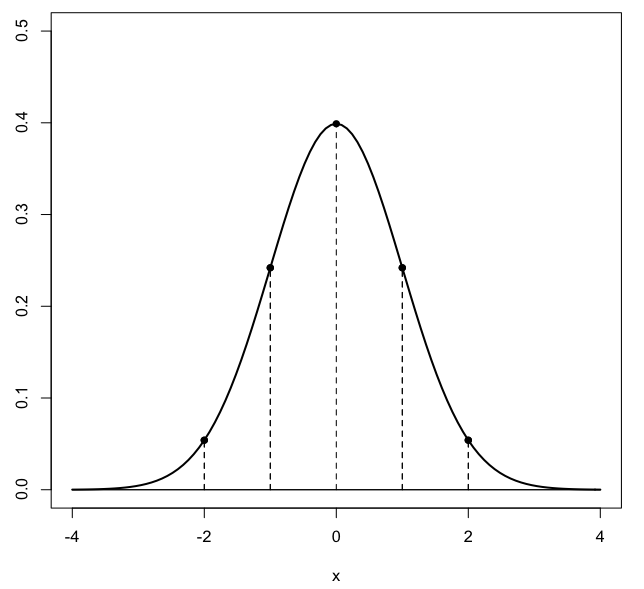
\includegraphics [scale=0.4] {gauss3.png} \end{center}

\title{Cubics}
\date{}

\begin{document}
\maketitle
\Large
Every cubic polynomial equation has at least one term containing $x^3$ but lacks any higher powers of $x$ such as $x^4$.

The general equation is
\[ y = ax^3 +  bx^2 + cx + d \]
and a typical graph ($x^3 - 3x^2 + x + 1$) looks something like this:
\begin{center} 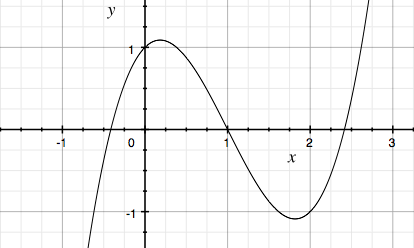
\includegraphics [scale=0.5] {cubic3.png} \end{center}
There is an axis of symmetry, here at $x = 1$, and the left half is the negative reflection of the right half about the value of $y = f(1) = 0$.

\subsection*{roots}

By the \emph{roots} of the equation, we mean those values of $x$ giving $y = 0$, that is, we are solving
\[ ax^3 +  bx^2 + cx + d = 0 \]

In this case we can always multiply through by $1/a$ so the term $x^3$ has a coefficient of $1$, and if we do that then the coefficients are often renamed as:
\[ x^3 + ax^2 + bx + c = 0 \]

The cubic is an odd function, so the sign of $x$ carries through in $x^3$.  Since the $x^3$ term dominates the value of the function for extreme values of $x$, when $x << 0$, $y$ is large and negative, while for $x >> 0$, $y$ is large and positive.  This is clearly seen for the above plot.

As a result, the graph of the function must cross the $x$-axis at least once, and thus every cubic has at least one real root, where $f(x) = 0$.  

From this we conclude that every cubic can be factored into 
\[ (x - r)(x^2 + sx + t)  \]
where $x = r$ is the guaranteed real root, although it isn't always the case that $r$ is an integer, of course.

This expression is equal to zero either when $x=r$ or when the quadratic term is zero.

The roots of a quadratic $x^2 + sx + t$ are given by the familiar
\[ \frac{-s \pm \sqrt{s^2 - 4t}}{2} \]

We know that quadratics have either two real roots or none depending on the value of the discriminant under the square root.  We consider the case of repeated roots (when the discriminant is zero) as \emph{two} roots.

Therefore, every cubic has either one real root or three of them.

Graphically, we can easily see the general truth of this statement.
\begin{center} 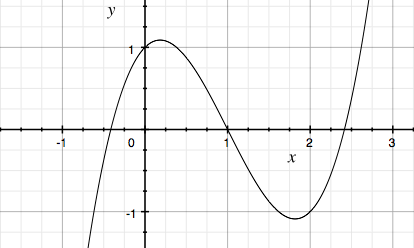
\includegraphics [scale=0.5] {cubic3.png} \end{center}

In this example from before, near $x=1.8$, no matter how far the graph goes below the $x$-axis before it turns the second time, we can add that much to the constant $c$.  The result will be that the graph just touches the $x$-axis at this point. A tiny bit more and it will not cross at all.

\begin{center} 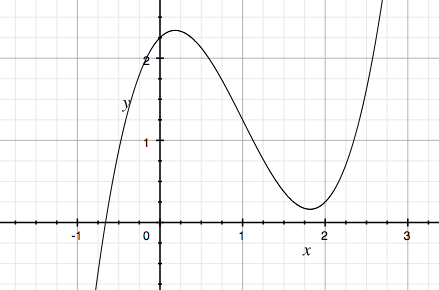
\includegraphics [scale=0.5] {cubic4.png} \end{center}
The above graph is the same equation but with $1.25$ added to $c$:  ($x^3 - 3x^2 + x + 2.25$).

\subsection*{factoring}

Every cubic has at least one real root and as a consequence, the solution where $y=0$ can be written as
\[ (x - r)(x^2 + sx + t) = 0 \]

Multiplying out
\[ = x^3 + (s - r)x^2 + (t - rs)x - rt   \]
Thus $a = s-r$ and $c = -rt$.

Suppose we know, or have guessed $r$.  We can find $s$ and $t$ by comparison with the original equation.

As an example, consider:
\[ (x - 1)(x + 1)(x + 2) = 0 \]
\[ = (x - 1)(x^2 + 3x + 2) \]
\[ = x^3 + 2x^2 + 5x - 2 \]
We plot this, guess that $x = 1$ is a root, check and find that $x = 1$ solves the equation.  Thus $r = 1$ and since
\[ c = -2 = -rt \]
then $t = 2$.  Also
\[ a = 2 = s - r = s - 1 \]
and $s = 3$.

Alternatively, there is a formalism called synthetic division for deriving $s$ and $t$.  I have a simple version of this I like better than the complete formal approach.  Consider
\[ x^3 - 5x^2 - 2x + 24 = 0 \]
Suppose we are given that $x = -2$ is a solution, which is easily checked.  Now write:

\[ x^3 - 5x^2 - 2x + 24 \]
\[ = (x + 2)(x^2 + \_\_\_ \ x + \_\_\_ ) = 0 \]

The cofactor of $x^2$, the first term on the right, is clearly just $1$, so that we get the desired $x^3$ in the product.

Then we see that, multiplying by $2$ we get $2 \times x^2 = 2x^2$, where the desired result is $-5x^2$.  We need another $-7x^2$.  Therefore the cofactor of $x$ on the right must be $-7$ so that $-7x^2 + 2x^2 = -5x^2$:
\[ (x + 2)(x^2 -7x + \_\_\_ ) = 0 \]

Then we see that, multiplying by $2$ we have $2 \times -7x = -14x$, where the desired result is $-2x$.  We need another $12x$.  Therefore, the constant term on the right must be $12$ so that $-14x + 12x = -2x$.
\[ (x + 2)(x^2 -7x + 12) = 0 \]

And finally, we check the whole thing, multiplying $2 \times 12$ to give the desired constant, $24$.  This must work out if we've done the rest correctly and $x = -2$ is really a solution.

Inspired guessing can help.  Consider

\[ x^3 - 4x^2 - 9x + 36 = 0 \]
You may notice that $a \times b = c$.  This tells us that $1 - 4$ is a factor of $-9 + 36$.  We guess that $x = 4$ is a solution:
\[ (x - 4) (x^2 + \_\_\_ \ x + \_\_\_ ) = 0 \]
We don't need anything more than $-4x^2$ so the cofactor of $x$ on the right is $0$ and write
\[ (x - 4) (x^2 + \_\_\_ ) = 0 \]
For the constant, we guess $-9$ so as to get $-9x$ and then check $-4 \times -9 = 36$.
\[ (x - 4) (x^2 - 9) = 0 \]
Finally, we can factor the second term
\[ (x - 4) (x + 3)(x - 3) = 0 \]

\subsection*{relating roots to cofactors}

Suppose a cubic has three distinct real roots, meaning there are real numbers $p,q,r$ such that
\[ (x - p)(x - q)(x - r) = 0 \]
Multiplying out we would obtain for the constant term:  $-pqr$.

\[ (x^2 - qx - px + pq)(x - r) = 0 \]
\[ x^3 - qx^2 - px^2 + pqx - rx^2 + qrx + prx - pqr = 0 \]
\[ x^3 - (p + q + r)x^2 + (pq + qr + pr)x - pqr = 0 \]

So
\[ d = -pqr \]
Furthermore
\[ a = - (p + q + r) \]
\[ b = pq + qr + pr \]

\emph{If there are three  real roots, they multiply to give the constant term.}
\[ (x - 1)(x + 2)(x + 1) \]
\[ = (x^2 + x - 2)(x + 1) \]
\[ = x^3 + 2x^2 - x - 2  \]
$1 \times -2 \times -1 = -2$. 

Actually, a related statement is true even if two of the roots are not real.  In principle, we can factor out the single real root, leaving a quadratic.

We said that the roots of a quadratic $x^2 + sx + t$ are given by
\[ \frac{-s \pm \sqrt{s^2 - 4t}}{2} \]

If the second and third roots are imaginary they are so because what is under the square root is negative, so the above can be written as
\[ z = u \pm iv \]
These consist of two complex numbers, which are complex conjugates.  Their product is a real number:
\[ (u + vi)(u - vi) = u^2 + v^2 \]

When we plug the three roots into $(x-p)(x-q)(x - r)$ we get
\[ (x - u + vi)(x - u - vi) (x-r) \]
\[ = x^2 -ux -vix - ux  + u^2 + uvi + vix - uvi + v^2)(x - r) \]
The imaginary terms with $i$ cancel.
\[ = (x^2 -2ux + u^2 + v^2)(x - r) \]
\[ = x^3 - 2ux^2 + u^2x + v^2x - rx^2 + 2urx - u^2r - v^2r \]
\[ = x^3 - (2u + r)x^2 + (u^2 + 2ur + v^2)x - r(u^2 + v^2) \]

The result is all real coefficients.
\[ d = - r(u^2 + v^2) \]
and $d$ is the product of the three roots.

\subsection*{extreme points}

The points where the graph turns around can be found by taking the derivative and setting it equal to zero.
\[ y = ax^3 +  bx^2 + cx + d \]
\[ \frac{dy}{dx} = 3ax^2 + 2bx + c = 0 \]
\[ x = \frac{-2b \pm \sqrt{4b^2 - 12ac}}{6a} \]

Not all cubics have a downward sloping segment.  This happens when the quadratic for the slope has no real roots, i.e. when the square root term is less than or equal to zero.  A simple example of this is when $b = 0$, such as
\[ y = x^3 \]

This obviously has 3 equal real roots, all zero.
\begin{center} 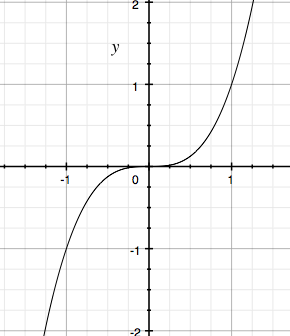
\includegraphics [scale=0.5] {cubic5.png} \end{center}
The slope is $2x^2$, which is never negative and equal to zero only at $x=0$.

\subsection*{repeated roots}
A cubic can have repeated roots.  Suppose
\[ (x - p)^2(x - q) = 0 \]
\[ = (x^2 - 2px + p^2)(x - q) \]
\[ = x^3 - qx^2 - 2px^2 + 2pqx + p^2 x - p^2q \]
\[ = x^3 - (q + 2p)x^2 + (2pq + p^2)x - p^2q \]
And, as before, the product of the roots is $-d$.

Graphically, two repeated roots means that one of the extreme points is also a root.

\[ (x+1)(x - 1)(x - 1) \]
\[ = (x + 1)(x^2 - 2x + 1) \]
\[ = x^3 - x^2 - x + 1  \]
\begin{center} 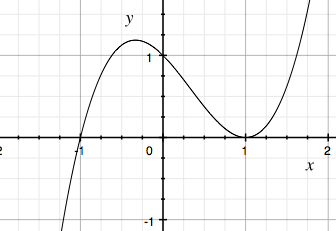
\includegraphics [scale=0.5] {cubic6.png} \end{center}

The slope is zero when
\[ 3x^2 -2(q + 2p)x + (2pq + p^2) = 0 \]

\subsection*{translation}
Continuing with $y = x^3$, when we add or subtract a value from $y$ the plot is shifted up or down, similarly, changes to $x$ shift the same curve to the left or right.

For example:
\[ (x - 1)^3 = x^3 - 3x^2 + 3x - 1 \]
What this means is that the cofactors $a$ and $b$ may be non-zero and the shape still be the same as $y = x^3$.  (The fact that $a, b, c$ conform to the cubic expansion is a tipoff, however).  The following section describes what is also essentially a horizontal translation.

\subsection*{depressed cubic}

Tartaglia discovered that the quadratic term can be removed from a cubic
\[ x^3 + ax^2 + bx + c \]

by an inspired substitution, $x = u - a/3$.  Actually, I find the arithmetic a bit confusing, so I will further substitute $v = a/3$ and so $x = u - v$.

\[ (u - v)^3 + a(u - v)^2 + b(u - v) + c \]

Now, expand each power of $u-v$ in order.  

The cubic binomial $(u - v)^3$ has cofactors of $3$ for the inner terms 

\[ (u-v)^3 = (u - v)(u^2 - 2uv + v^2) \]
\[  = u^3 - 2u^2v + uv^2 - u^2v + 2uv^2 - v^3 \]
\[  = u^3 - 3u^2v + 3uv^2 - v^3 \]
Switch the order so that the power of $u$ is last in each term
\[ = u^3  - 3vu^2 + 3v^2u - v^3 \]

The quadratic is
\[ a(u - v)^2 = a \ [ \ u^2 - 2uv + v^2 \ ] \]
\[ = au^2 - 2avu + av^2 \]

The linear term is just $bu - bv$.  

Finally, collecting all the terms and grouping them by powers of $u$
\[ = u^3 \ [ \ - 3v + a \ ] \ u^2  + \ [ \ 3v^2 - 2av + b \ ] \ u + \ [ \ - v^3 + av^2 - bv + c  \ ] \]

The bright idea is that the cofactor of $u^2$
\[ - 3v + a \]
 is equal to zero by the terms of the substitution ($v = a/3$).

That leaves:
\[ = u^3 + \ [ \ 3v^2 - 2av + b \ ] \ u + \ [ \ - v^3 + av^2 - bv + c  \ ] \]

If we write 
\[ m = 3v^2 - 2av + b \]
\[ n = - v^3 + av^2 - bv + c \]
then the cubic is
\[ u^3 + mu + n = 0 \]

We can reverse the second substitution ($v = a/3$).  We have one less term in each formula, which is simplified a bit, but this also makes the formulas more awkward.

\[ m = 3\frac{a^2}{3^2} - 2a\frac{a}{3} = \frac{a^2}{3} - 2\frac{a^2}{3} = - \frac{a^2}{3} + b  \]
and 
\[ n = -\frac{a^3}{3^3} + a \frac{a^2}{3^2} - \frac{ab}{3} + c \]
\[ =  2 \frac{a^3}{3^3} -\frac{ab}{3} + c \]

Here's an example.  Consider:
\[ x^3 + 3x^2 - x + 1 = 0 \]

\[ a = 3, \ \ \ \ b = -1, \ \ \ \ c = 1 \]
So 
\[ m = - \frac{a^2}{3} + b = - \frac{a^2}{3} - 1 = -4 \]
The constant $n$ is
\[  n = \frac{2a^3}{3^3} - \frac{ab}{3} + c \]
\[ 2 + 1 + 1 = 4 \]
So the transformed version is
\[ u^3 - 4u + 4 \]
And this is indeed the same curve, simply displaced to the right by 1 unit, as the substitution $x = u - a/3$ or $x = u -1$ implies.

\begin{center} 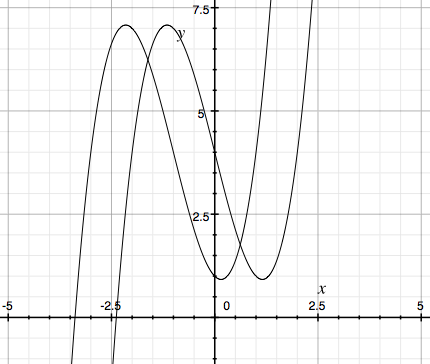
\includegraphics [scale=0.5] {cubic7.png} \end{center}
The real root is also the same (taking into account the translation).

An example from Nahin is
\[ x^3 - 15x^2 + 81x - 175 = 0 \]

The coefficient of $u$ is
\[ (-\frac{a^2}{3} + b) \]
\[ = -\frac{(-15)^2}{3} + 81 = -75 + 81 = 6 \]
The constant is
\[ \frac{2a^3}{3^3} - \frac{ab}{3} + c \]
\[ = \frac{2(-15)^3}{3^3} - \frac{(-15)81}{3} - 175 \]
\[ = -150 + 405 - 175 =  -20 \]
Hence we have
\[ u^3 + 6u - 20 = 0 \]
By trial and error, we find that $u = 2$ is a solution.

Reversing the substitution, $3v = a$.  This is the cofactor of $x^2$, the $a$ from the original equation!  So $v = a/3 = -15/3 = -5$.

Thus $x = u - v = 2 - (-5) = 7$.  Check by substitution:
\[ (7)^3 - 15(7^2) + 81(7) - 175 = 0 \]
Factor out $7$
\[ 7^2 - 15(7) + 81 - 25 = 0 \]
\[ 49 - 105 + 81 - 25 = 0 \]
which checks.

The resulting equation (lacking a quadratic term), is called a \emph{depressed} cubic.
\[ u^3 + mu + n = 0 \]

The result is kind of amazing.  For any cubic containing $ax^2$, we can obtain the same curve without any quadratic term.

\subsection*{form of the curve}
The constant simply displaces $y$ by some value.  The coefficient of $x^3$ stretches the curve.

From consideration of the depressed quadratic, you can see that the essential form is conferred by the cofactor of $x$ in, say
\[ y = x^3 - 3x \]
\begin{center} 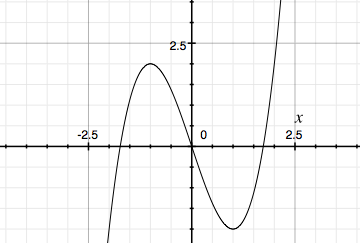
\includegraphics [scale=0.5] {cubic8.png} \end{center}

The larger the value of $b$, the bigger the deviations before the curve turns back.  It's curious that the extreme points are exactly $y = 2$ here.  That's because
\[ \frac{dy}{dx} = 3x^2 - 3 = x^2 -1 \]
Hence they occur at $x = \pm 1$, where $y = \pm 2$.

In an expression like $y = x^3 + ax^2 + bx + c$, increasing $a$ makes the central displacement more pronounced, while increasing $b$ makes it less pronounced.   Interestingly, having all three constants equal to $1$ makes it go away altogether.
\[ y = x^3 + x^2 + x + 1 \]
\begin{center} 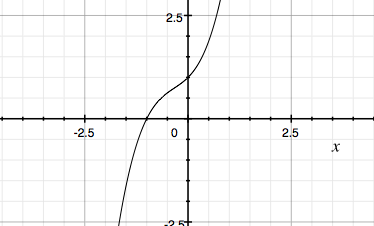
\includegraphics [scale=0.5] {cubic9.png} \end{center}
$x = -1$ has solution $y = 0$, and that's the single real root because
\[ x^3 + x^2 + x + 1 = (x  + 1)(x^2 + 1) \]
and we know $x^2 + 1$ has $i = \pm \sqrt{-1}$ as its solution.

Also, we note for this example
\[ y = x^3 + x^2 + x + 1 \]
Get the slope as the derivative and set it equal to zero:
\[ y' = 3x^2 + 2x + 1 = 0 \]
for which the roots are
\[ x = \frac{-2 \pm \sqrt{4 - 12}}{6} \]
The discriminant is negative, so there is no $x$ that gives a slope of zero.

The minimum value of $y'$ is $y'' = 0$
\[ y'' = 6x + 2 = 0 \]
\[ x = -\frac{1}{3} \]
\[ y' = \frac{3}{9} - \frac{2}{3} + 1 = \frac{2}{3} \]

\subsection*{Solving the depressed cubic}

Which brings us finally to Cardano, and the solution of the cubic.

Dunham has a picture of the geometrical division of a cube that Cardano visualized, 
\begin{center} 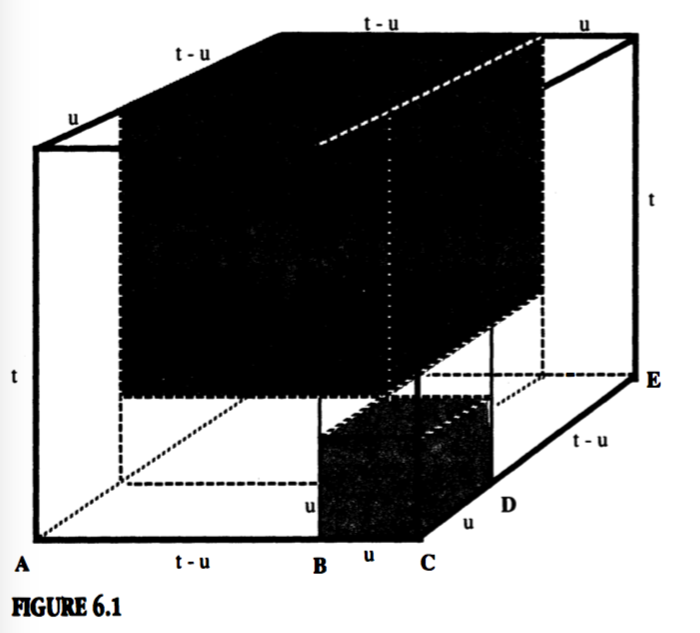
\includegraphics [scale=0.3] {cubic10.png} \end{center}

However, with modern notation, we can get there pretty simply from algebra.
\[ (t - u)^3 = t^3 - 3t^2u + 3tu^2 - u^3 \]
\[ (t - u)^3 + 3t^2u - 3tu^2 = t^3 - u^3 \]
\[ (t-u)^3 + 3ut(t - u) = t^3 - u^3 \]

Now let $x = t - u$
\[ x^3 + 3tux = t^3 - u^3 \]
Substitute $m = 3tu$ and $n = t^3 - u^3$:
\[ x^3 + mx = n \]

This is a depressed cubic.
\[ x^3 + mx - n = 0 \]

The idea is to start with a depressed cubic we want to solve, and use that to get values for $m$ and $n$.  

If we can then determine values for $t$ and $u$, $x = t - u$ will be the solution that we seek.

We have the two conditions:  $m = 3tu$ and $n = t^3 - u^3$.  Solve the first for $u$ \[ u = \frac{m}{3t} \]
and substitute into the second:
\[ n = t^3 - \frac{m^3}{(3t)^3} \]
Multiply both sides by $t^3$
\[ nt^3 = t^6 - \frac{m^3}{27} \]

Looks like it's getting more complicated.

But this is a quadratic equation in disguise!
\[ t^6 - nt^3 - \frac{m^3}{27} = 0 \]

By the quadratic formula:
\[ t^3 = \frac{n \pm \sqrt{n^2 + 4m^3/27}}{2} \]
Take the positive square root 
\[ = \frac{n}{2} + \sqrt{\frac{n^2}{4} + \frac{m^3}{27}} \]
and take its cube root:
\[ t = \ [ \ \frac{n}{2} + \sqrt{\frac{n^2}{4} + \frac{m^3}{27}} \ ]^{1/3} \]

Since $u^3 = t^3 - n$, just subtract $n$ from the expression for $t^3$ before taking the cube root.  
\[ u = \ [ \ -\frac{n}{2} + \sqrt{\frac{n^2}{4} + \frac{m^3}{27}} \ ]^{1/3} \]

Then
\[ x = t - u \]
\[ =  [ \ \frac{n}{2} + \sqrt{\frac{n^2}{4} + \frac{m^3}{27}} \ ]^{1/3} -  \ [ \ -\frac{n}{2} + \sqrt{\frac{n^2}{4} + \frac{m^3}{27}} \ ]^{1/3} \]

We can write this more simply by pre-computing
\[ r = \frac{n}{2}, \ \ \ \  s = \frac{m^3}{27} \]
Then
\[ x = \ [ \ r + \sqrt{r^2 + s} \ ]^{1/3} - \ [ \ -r + \sqrt{r^2 + s} \ ]^{1/3} \]

Here is Cardano (recall we are solving $x^3 + mx - n = 0$):

\begin{quote}
Cube one-third the coefficient of x; add to it the square of one-half the con­stant of the equation; and take the square root of the whole. You will dupli­cate [repeat] this, and to one of the two you add one-half the number you have already squared and from the other you subtract one-half the same . . . Then, subtracting the cube root of the first from the cube root of the second, the remainder which is left is the value of x.
\end{quote}

\subsection*{example}
How about Cardano's example:
\[ x^3 + 6x - 20 = 0 \]
Clearly, $2$ is a solution to this.  It is the only real root.

We have $m = 6$ and $n = 20$, so $n/2 = 10$.

$m = 6$ so
\[ \frac{m^3}{27} = \frac{6^3}{27} = \frac{(2 \cdot 3)^3}{3^3} = 2^3 = 8  \]
and then
\[ x = \ [ \ 10 + \sqrt{100 + 8} \ ]^{1/3} - \ [ \ -10 + \sqrt{100 + 8} \ ]^{1/3} \]
These two terms are
\[ (10 + \sqrt{108})^{1/3} = 2.732 \]
\[ (-10 + \sqrt{108})^{1/3} = 0.732 \]
The difference is indeed very close to $2$.

\subsection*{example 2}
Another famous example is
\[ x^3 - 15x - 4 = 0 \]
Guessing, we obtain $x = 4$ as one root.

Now, to factor out $(x - 4)$:
\[ x^3 - 15x - 4 = (x - 4) (\_\_\_ \ x^2 + \_\_\_ \ x + \_\_\_ ) \]
\[ x^3 - 15x - 4 = (x - 4) (x^2 + \_\_\_ \ x + \_\_\_ ) \]
\[ x^3 - 15x - 4 = (x - 4) (x^2 + 4x + \_\_\_ ) \]
\[ x^3 - 15x - 4 = (x - 4) (x^2 + 4x + 1 ) \]
The last multiplication to give the constant works, which provides a check on the whole thing.

We solve the quadratic as
\[ x = \frac{-4 \pm \sqrt{16 - 4}}{2} = -2 \pm \sqrt{4 - 1} = -2 \pm \sqrt{3} \]

Check the positive root:
\[ (-2 + \sqrt{3})^2 + 4 (-2 + \sqrt{3}) + 1 \]
\[ = 4 - 4 \sqrt{3} + 3 - 8 + 4 \sqrt{3} + 1 \]
\[ = 0 \]

So we have three real roots.  Notice that
\[ 4 + (-2 + \sqrt{3} ) + (-2 - \sqrt{3} ) = 0 \]
The sum of the roots is zero.

Now use Cardano's solution to solve
\[ x^3 - 15x - 4 \]
First
\[ r = \frac{n}{2} = -2 \]
\[ s = \frac{m^3}{27} =  \frac{-15^3}{27} = -125 \]

\[ x = \ [ \ r + \sqrt{r^2 + s} \ ]^{1/3} - \ [ \ -r + \sqrt{r^2 + s} \ ]^{1/3} \]
\[ = \ [ \ -2 + \sqrt{4 + -125} \ ]^{1/3} - \ [ \ 2 + \sqrt{4 + -125} \ ]^{1/3} \]
\[ = \ [ \ -2 + \sqrt{-121} \ ]^{1/3} - \ [ \ 2 + \sqrt{-121} \ ]^{1/3} \]
\[ = \ [ \ -2 + \sqrt{-121} \ ]^{1/3} + \ [ \ - 2 - \sqrt{-121} \ ]^{1/3} \]

That seems strange at first.  We have three real roots, but Cardano's solution gives an expression which is the sum of two imaginary numbers.

The resolution is that the two numbers here are complex conjugates.  What we have is
\[ \ [ \ z \ ]^{1/3} + \ [ \ z* \ ]^{1/3} \]
where
\[ z = -2 + 11 i \]
If we write this in polar form
\[ z = re^{i\theta} \]
\[ z* = re^{-i \theta} \]
so
\[ z^{1/3} = r^{1/3} e^{i \theta/3} \]
\[ z*^{1/3} =  r^{1/3} e^{i(-\theta/3)} \]
The sum is
\[ r^{1/3} \ [ \ e^{i \theta/3} + e^{i(-\theta/3)}  \ ] \]
The term in the brackets is the sum of a complex number and its complex conjugate, $w + w*$, which is completely real, so the whole thing is completely real.

\[ e^{i \theta/3} + e^{i(-\theta/3)} = 2 \cos \ (\theta/3) \]

To actually do the calculation
\[ z = -2 + 11 i \]
\[ zz* = (-2 + 11i)(-2 - 11i) = -4 + 121 \]
\[ r = \sqrt{zz*} = \sqrt{117} \]
\[ r^{1/3} = 2.211 \]

For the angle
\[ \theta = \tan^{-1} -\frac{11}{2} = - 1.391 \]
\[ \theta/3 =  - 0.46 \]
The term in the brackets is
\[ 2 \cos \ (\theta/3) = 2 \cos \ (- 0.46) = 1.788  \]

The whole thing is
\[ r^{1/3} \ [ \ e^{i \theta/3} + e^{i(-\theta/3)}  \ ]  = 2.211(1.788) \approx 4  \]

A much simpler method is to notice that
\[ (2 + \sqrt{-1})^3 = (2 + \sqrt{-1}) (4 + 4 \sqrt{-1} - 1) \]
\[ =  (2 + \sqrt{-1}) (3 + 4 \sqrt{-1} ) \]
\[ = 6 + 3  \sqrt{-1} + 8  \sqrt{-1} - 4 \]
\[ = 2 + 11 \sqrt{-1} = 2 + \sqrt{-121} \]
The same result is obtained with $-2 + \sqrt{-1})^3$.

Hence 
\[ x = \ [ \ -2 + \sqrt{-121} \ ]^{1/3} - \ [ \ 2 + \sqrt{-121} \ ]^{1/3} \]
\[ = 2 + 2 = 4 \]

\subsection*{example 3}
\[ x^3 + 3x - 2 = 0 \]

It might be simplest to try $m=3$ and $n = 2$, so $n/2 = 1$.

$m = 3$ so
\[ \frac{m^3}{27} = 1  \]
Then
\[ x = \ [ \ 1 + \sqrt{2} \ ]^{1/3} - \ [ \ -1 + \sqrt{2} \ ]^{1/3} \]
These two terms are 
\[ = 1.3415 - 0.745 = 0.596  \]
This doesn't quite match the plot, however (which is closer to 0.7).

The arithmetic is tiresome, so write a script to do it.

\subsection*{script}

\begin{verbatim}
# Cardano's method for solving
# x^3 + mx = n 

import sys
from math import sqrt

def simplify(a,b,c):
    f = 1.0*a/3
    g = a*f   # a^2/3
    m = -g + b
    h = f*g   # a^3/3^2
    j = h/3   # a^3/3^3
    return m, (-j + h - (a*b*1.0)/3 + c)

def cardano(m,n):
    c = (m**3)/27
    h = n/2.0
    r = 0.3333333333

    rad1 = ( h + sqrt(h**2 + c))
    rad2 = (-h + sqrt(h**2 + c))
    return round(rad1**r - rad2**r, 5)
\end{verbatim}

\begin{verbatim}
> python
..
>>> from cubics import *
>>> simplify(3,-1,1)
(-4.0, 4.0)
>>> cardano(6,20)
2.0
>>> cardano(3,2)
0.59607

\end{verbatim}

We get Cardano's result, and confirm the calculation for the second example.  This suggests that the error lies in the plotting program.

\subsection*{practical solving}

A practical approach to real problems involves first plotting the function so as to know whether there is one real root or three, and get an idea of their values.

For example

\textbf{plotter.py}

\begin{verbatim}
from matplotlib import pyplot as plt
import numpy as np

def plot(X,Y):
    plt.scatter(X,Y,s=5)
    plt.axhline()
    plt.axvline()
    #plt.axes().set_aspect('equal')
    plt.savefig('x.png')

def cubic(a,b,c,d):
    def f(x):
        return a*x**3 + b*x**2 + c*x + d
    L = np.linspace(-10,10,2000)
    X = list()
    Y = list()
    for x in L:
        y = f(x)
        if y < -10 or y > 10:
            continue 
        X.append(x)
        Y.append(y)
    plot(X,Y)

cubic(1,1,1,1)
\end{verbatim}

\begin{center} 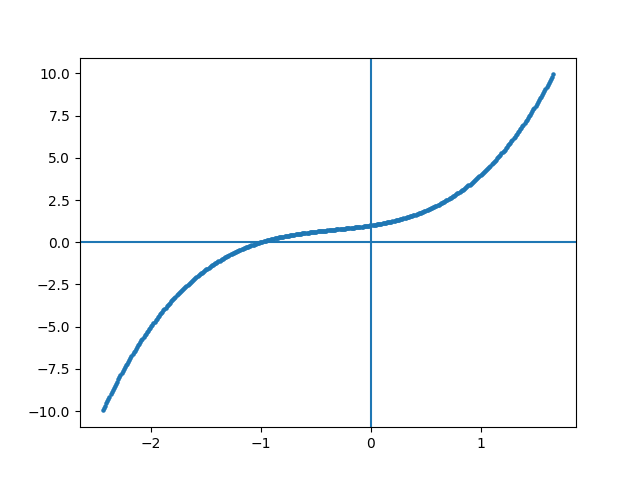
\includegraphics [scale=0.5] {cubic11.png} \end{center}

An actual solver might look something like this:

\textbf{guess.py}

\begin{verbatim}
import numpy as np

a,b,c = 1, 1, 1

def f(x):
    return x**3 + a*x**2 + b*x + c

def getX(x1,x2):
    N = 1000
    return np.linspace(x1,x2,N)

# assumes we go from f(x) < 0 to f(x) > 0
def guess(x1, x2):
    std_order = f(x1) < f(x2)
    
    print 'guess'
    print 'x1 = ', str(x1)
    print 'x2 = ', str(x2)
    print 'y1 = ', str(f(x1))
    print 'y2 = ', str(f(x2))
    print
    
    X = getX(x1,x2)
    if not std_order:
        X.reverse()
    assert f(X[0]) < 0 and f(X[-1]) > 0
    
    for i,x1 in enumerate(X):
        x2 = X[i+1]
        # must happen
        if f(x2) > 0:
            if not std_order:
                return x2, x1
            return x1, x2
     
def close(r):
    e = 1e-12
    return not (r > e or r < -e)
    
x1 = -2
x2 =  0
i = 0

while i < 100:
    print i+1
    x1, x2 = guess(x1, x2)
    if close(x2 - x1):
        break
    i += 1
\end{verbatim}

\textbf{output}

\begin{verbatim}
> python guess.py
1
guess
x1 =  -2
x2 =  0
y1 =  -5
y2 =  1

2
guess
x1 =  -1.001001001
x2 =  -0.998998998999
y1 =  -0.00200400701102
y2 =  0.001999998999

3
guess
x1 =  -1.000001002
x2 =  -0.999998997997
y1 =  -2.00400801575e-06
y2 =  2.00400399997e-06

4
guess
x1 =  -1.000000001
x2 =  -0.999999998997
y1 =  -2.00601180111e-09
y2 =  2.00601202316e-09

5
guess
x1 =  -1.0
x2 =  -0.999999999999
y1 =  -2.00772731773e-12
y2 =  2.00817140694e-12

> 
\end{verbatim}

It's pretty clear that $x = -1$ is the real root.
\[ x^3 + x^2 + x + 1 = (x + 1)(x^2 + 1) \]
The product of the two other roots is $x^2 + 1$, that is, they are $\pm \ i$.

Recall that $d = -pqr$ so
\[ d = - \ [ \ (-1) \times i \times -i \ ] = - \ [ \ (-1) \times 1\ ] = 1 \]

\end{document}